% -*- mode:latex; mode:flyspell -*-
\subsection{Generating the task graph}
\label{sec:build-appl-graph}

\begin{figure*}[t!]
  \centering
  % 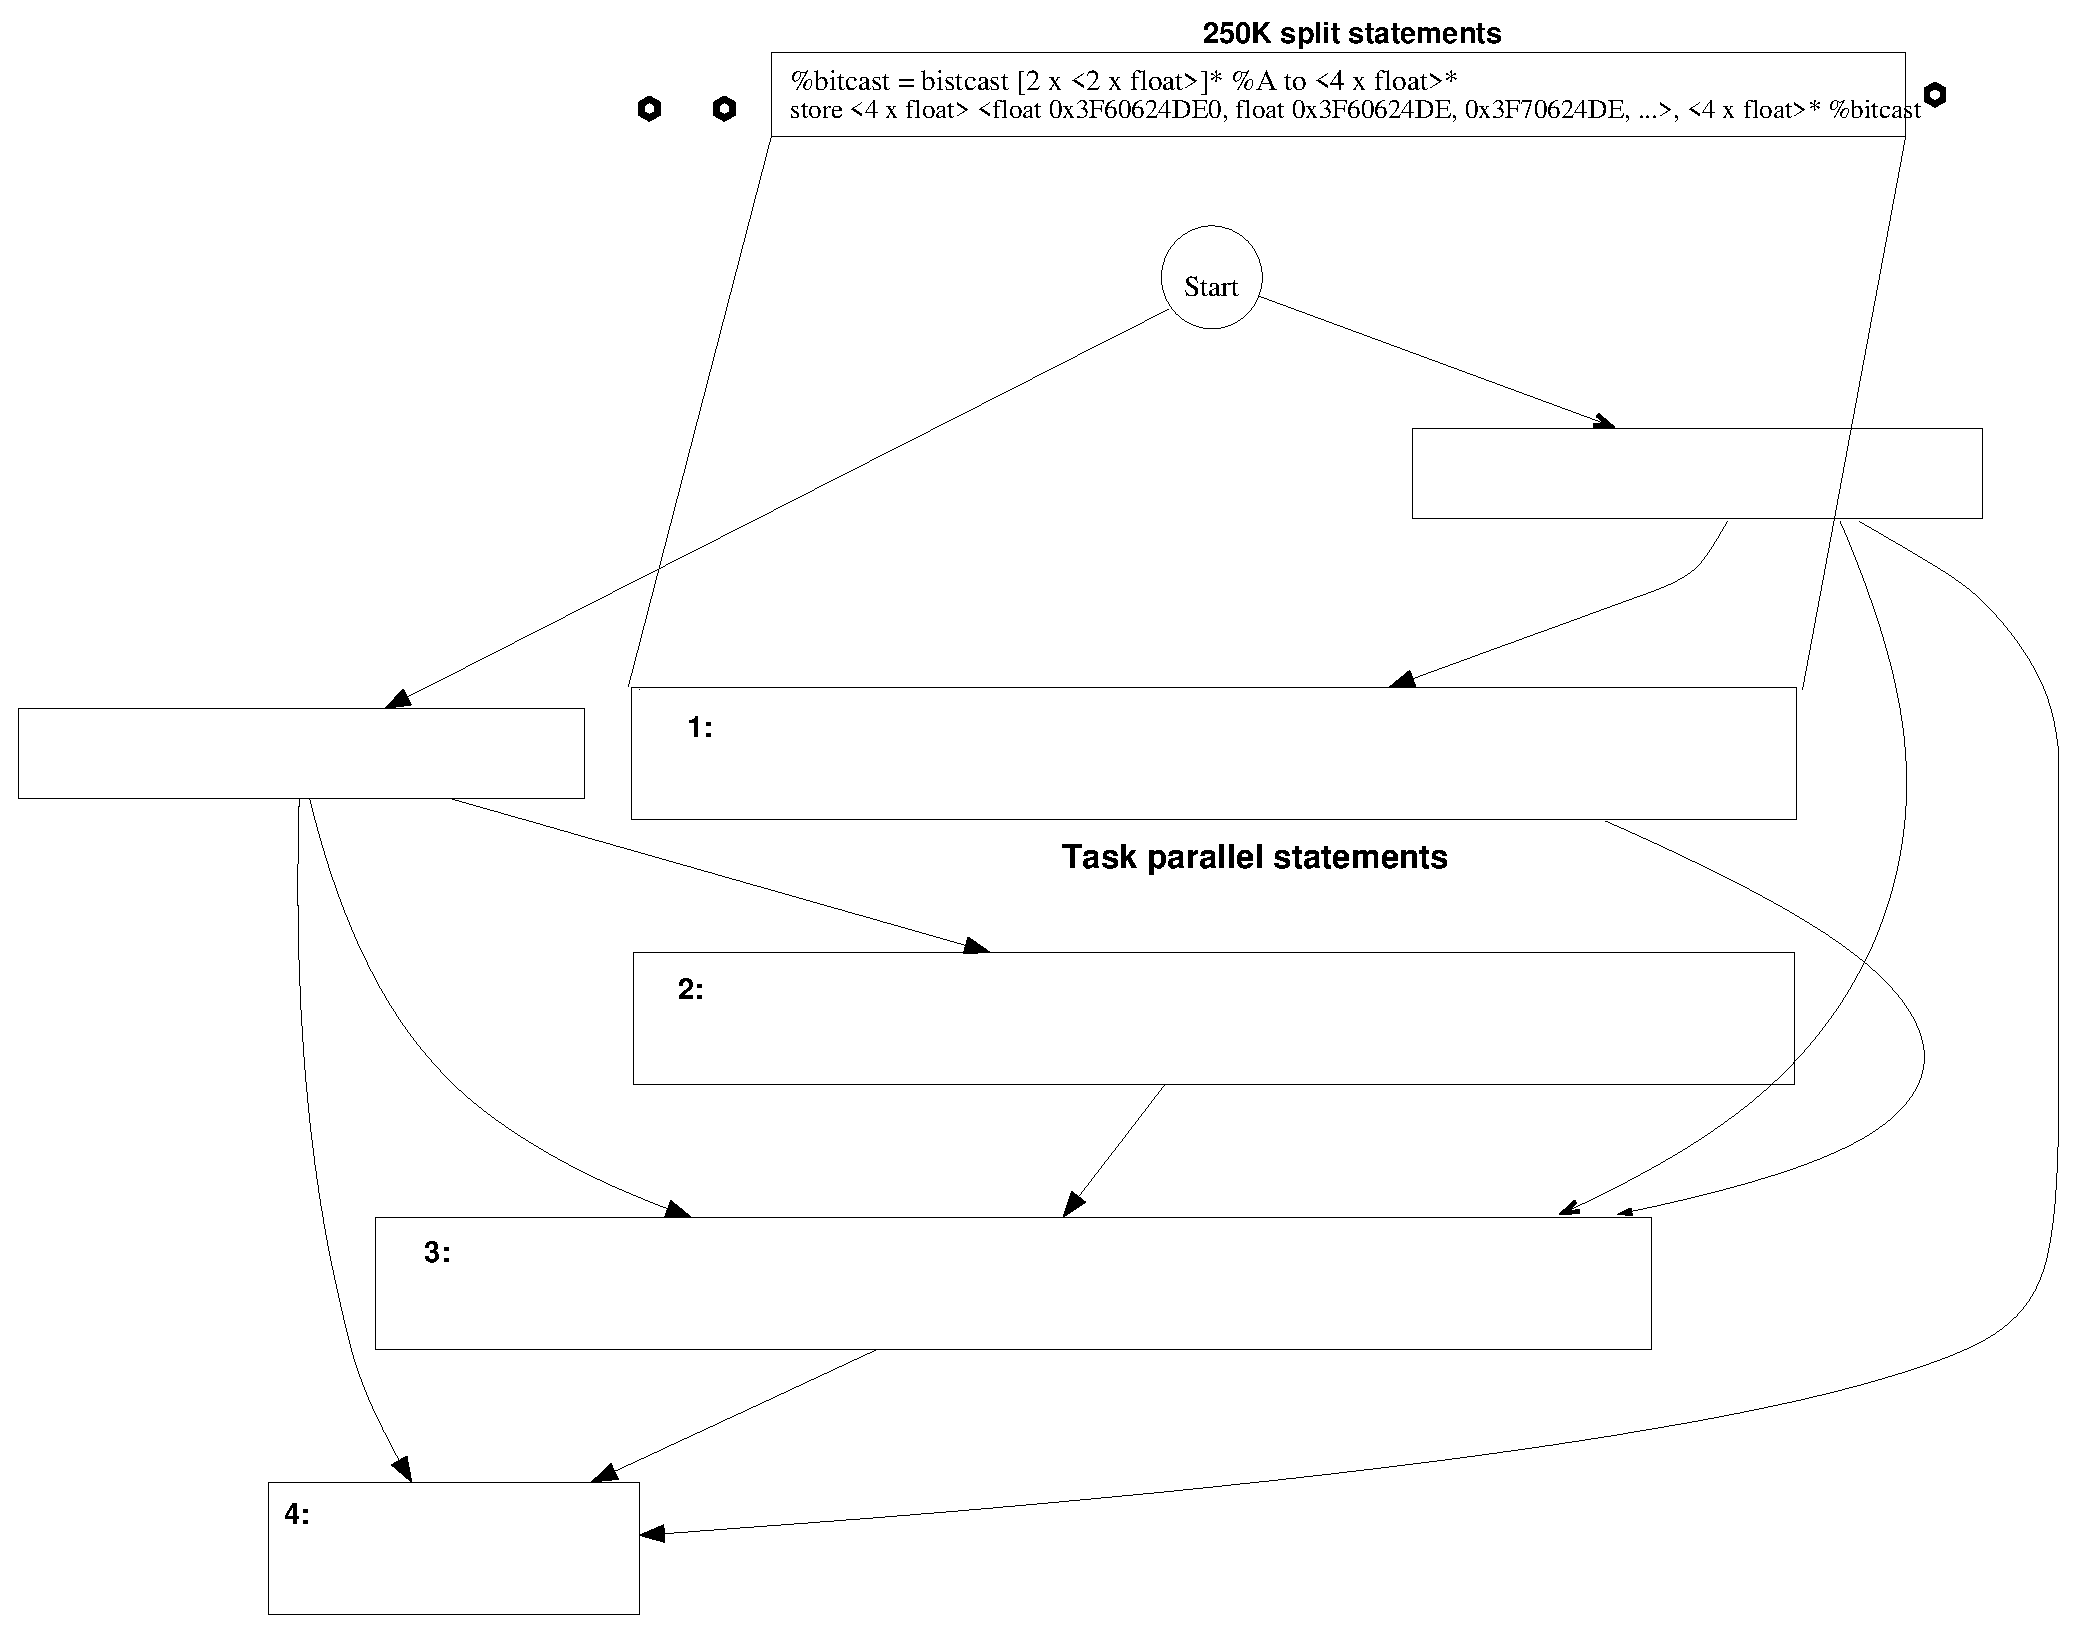
\includegraphics[scale=0.42]{./figures/jacobi2d}
  \scalebox{0.37}{\input{./figures/jacobi2d.pstex_t}}
  \caption{The task graph for the Jacobi example}
  \label{fig:1}
\end{figure*}

\begin{figure*}[t!]
  \centering
\begin{verbatim}
 %scevgep = getelementptr [1000 x <1000 x float>]* %A, i64 0, i64 %3
 %scevgep10 = bitcast <1000 x float>* %scevgep to i8*
 %ugep = getelementptr i8* %scevgep10, i64 4
 %scevgep11 = getelementptr [1000 x <1000 x float>]* %B, i64 0, i64 %3
 %scevgep1112 = bitcast <1000 x float>* %scevgep11 to i8*
 %ugep13 = getelementptr i8* %scevgep1112, i64 4
 call void @llvm.memcpy.p0i8.p0i8.i64(i8* %ugep,i8* %ugep13,i64 3996,i32 4,i1 false)
\end{verbatim}
  \caption{LLVM code for assignment statement \texttt{4} from
    Figure~\ref{fig:2}}
  \label{fig:3}
\end{figure*}

The task graph is built from the application by the compiler % extracts
% task and data parallelism form the application for partitioning the
% application onto the architecture. The compiler looks at every
% statement in the program to form the task graph. The task graph is
% formed
in the
following manner:

\begin{itemize}

\item The assembly instruction count for every statement is obtained
  first. Currently, we look at the LLVM (Low level virtual
  machine)~\cite{clat04} instruction count. For example, the LLVM code
  generated for the assignment statement \texttt{4} in
  Figure~\ref{fig:2} is shown in Figure~\ref{fig:3}. The LLVM
  instruction count gives an approximation of the instruction count of
  the underlying hardware, while remaining independent of the hardware
  itself.

\item Every loop is fissed (split into multiple loops) thereby forming
  multiple statements. The intuition behind fissing the loops is two
  fold: (a) task parallelism can be exploited by running independent
  loop statements separately on different machines (see
  Figure~\ref{fig:1}, where statements \texttt{1} and \texttt{2} are
  split statements) and (b) the graph partitioner would give us feedback
  on the vector size of the loop, which can then be fused back if
  allocated to the same resource.

\item The vector counts for each statement is determined using
  dependence analysis and using the polyhedral model~\cite{mgri98}. The
  largest vector size requirement is given as the second requirement
  ($T^i_1$) in the task graph.

\item The polyhedral model is also used to find the iteration count of
  the statements and to determine the total amount of data (in bits)
  required to process by that statement. For example, statement
  \texttt{4} (the last \texttt{boxed} statement in Figure~\ref{fig:1})
  requires \texttt{7.8085KB} of data, while the first two statements
  \texttt{1} and \texttt{2} require 64-bits more due to the difference
  in the loop iteration count (see Figure~\ref{fig:2}).

\item The edges in Figure~\ref{fig:1} with 0 weights are dependence
  arcs. For example, in the Jacobi example, statements \texttt{1} and
  \texttt{2} can be carried out in parallel, while statements
  \texttt{3} and \texttt{4} have a dependence on these two statements
  and hence, cannot be split.

\end{itemize}

\paragraph{\textbf{Tiling vectors}}
\label{sec:tiling-vector-counts}

As we can see from Figure~\ref{fig:1}, three of the statements in Jacobi
example require almost a million vector instructions to be carried out
in parallel. The vector counts can increase quite quickly for large
examples (notice that the current 1 million vector count is just for a
small 1000 $\times$ 1000 Jacobi matrix). In order to properly utilize
the underlying vector hardware these vector lengths need to be split
into smaller vector lengths. The resultant vector lengths depend upon
the underlying hardware. Splitting the vector constraints is termed
tiling in the compiler community. There are many ways to tile a
vector. For example, given a single processing element with a small
vector size, a vector might be tiled to fit the underlying hardware
vector size and then run in a loop (an approach taken by the gcc
compiler). If a number of processing elements with differing vector
sizes are available as in the case of HPC architectures determining the
optimal vector tiles is a challenge and can be solved with
\textit{simulated annealing} (SA)~\cite{tbra01} or \textit{genetic
  algorithm} (GA)~\cite{tbra01} heuristics. In this article we do not
solve the problem of determining the tile sizes. Instead our framework
allows the application designers to plug and play with different vector
tiles in order to determine the tile size that suits their
architecture. We randomly generate different tile sizes for
experimentation.

An example tiling with 250K separate, 2 $\times$ 2 tiles for statement
\texttt{1} is shown in Figure~\ref{fig:1} with its resultant LLVM
code. It is important to mention that vectors are only single
dimensional. In Figure~\ref{fig:1}, we are type-casting a 2D matrix of
size 2 $\times$ 2 into a single dimensional 4 element vector. Such
vectorization is also called loop-collapsed vectorization, i.e., instead
of just vectorizing the inner most loop in Figure~\ref{fig:2} statement
\texttt{1}, we are collapsing the outer and inner loop into a single
vector instruction to improve performance. Such loop collapse is not
necessary and can be considered a super optimization. However, our
framework allows the application designers to explore such
possibilities.



%%% Local Variables:
%%% mode: latex
%%% TeX-master: "bare_conf"
%%% End:
